\subsection*{Hệ lập phương}
\begin{enumerate}[label=(\alph*)]
    \item Bằng việc coi gần đúng các rãnh gãy như các đường thẳng, ta ước lượng được chu vi của "hình tam giác" được tạo bởi các rãnh gãy \begin{equation}l\approx 55mm.\end{equation}
    Thể tích trung bình chiếm bởi một phân tử chính là thể tích của một ô lập phương cơ sở, được cho bởi \begin{equation}(2r)^3=\frac{M_{SiO_2}\times1\text{mol}}{N_A\rho}.\end{equation} Do đó tiết diện một ô mạng cơ sở là \begin{equation}S=(2r)^2=\left(\frac{M_{SiO_2}}{N_A\rho}\right)^{2/3}.\end{equation}
    Dựa vào đó ta ước lượng tổng số liên kết bị gãy: \begin{equation}N=\frac{\text{Tiết diện mặt gãy}}{\text{Tiết diện một ô mạng cơ sở}}=\frac{lc}{S}\approx 4\times 10^{14}\text{~liên kết}. \end{equation}
    \item Ẩn nhiệt hoá hơi là mật độ năng lượng để làm bay hơi thuỷ tinh. Như vậy, cần phải bẻ gãy hết các liên kết của thuỷ tinh. Xét hình lập phương có $n=p\times p\times p$ phân tử. Khi đó, ta thấy có $(p-1)\times(p-1)\times(p-1)$ liên kết theo mỗi hướng. Có ba hướng $(x,y,z)$ mà các liên kết nằm dọc theo cho nên có tổng cộng $3(p-1)^3=3(p^3-3p^2+p-1)$ liên kết. Với $p$ rất lớn, số hạng bậc ba trở nên áp đảo và  số liên kết xấp xỉ $3p^3=(6/2)n$; ở đây số hạng bậc ba đại diện cho liên kết giữa các phân tử nằm trong lòng khối thuỷ tinh, trong khi số hạng bậc hai và một biểu diễn liên kết của các phân tử nằm trên bề mặt và ở cạnh của hình khối. Một phân tử có thể liên kết với $A=6$ phân tử khác, nhưng số liên kết hiệu dụng chỉ bằng $A/2$ vì khi một liên kết được dùng chung bởi hai phân tử. \newline
    Ta có thể tiếp tục tổng quát hoá cách đếm  áp dụng cho mọi hình khối của ô cơ sở như sau: năng lượng liên kết giữa hai phân tử bất kì lần lượt có vị trí \(\mathbf r_i\) và \(\mathbf r_j\) trong không gian được biểu diễn bằng một hàm thế năng tương tác $U(\mathbf r_i, \mathbf r_j)$ chỉ phụ thuộc vào khoảng cách tương đối giữa chúng, tức $U(\mathbf r_i, \mathbf r_j)=U(\lvert \mathbf r_i -\mathbf r_j\rvert)$. Để cho gọn ta chỉ kỉ hiệu là $U_{ij}$, và biết rằng $U_{ij}=U_{ji}$. Lúc này tổng năng lượng liên kết của cả hệ $n$ phân tử chính là tổng thế năng tương tác giữa các phân tử cho bởi \begin{equation}U=U_{12}+U_{13}+\cdots U_{1n}+U_{23}+\cdots+U_{2n}+\cdots+U_{(n-1)n}=\sum_{\substack{i,j \\ i<j}}U_{ij}.\end{equation} Biến đổi đại số tiếp theo được thực hiện như sau \begin{equation}\sum_{\substack{i,j \\ i<j}}U_{ij}=\sum_{\substack{i,j\\i\neq j}}U_{ij}-\sum_{\substack{i,j \\ i>j}}U_{ij}=\sum_{\substack{i,j\\i\neq j}}U_{ij}-\sum_{\substack{i,j \\ i>j}}U_{ji}.\end{equation} Vai trò của hai chỉ số $i,j$ là tương đương cho nên \begin{equation}\sum_{\substack{i,j \\ i>j}}U_{ji}=\sum_{\substack{i,j \\ i<j}}U_{ij}.\end{equation} Như vậy, \begin{equation}\label{2_eq1.8}U=\sum_{\substack{i,j \\ i<j}}U_{ij}=\frac{1}{2}\sum_{\substack{i,j \\ i\neq j}}U_{ij}.\end{equation}  Ngay lúc đầu ta đã giả định rằng năng lượng liên kết chỉ đáng kể đối với các cặp phân tử liền kề (và cùng bằng $E_b$), thành thử \begin{equation}\label{eq2_1.9}
        U=\frac{1}{2}n(AE_b).\end{equation}  Trong việc đi từ phương trình \ref{2_eq1.8} tới phương trình \ref{eq2_1.9}, ta đã chỉ xét đến liên kết của các phân tử nằm trong lòng khối chất. Điều này hoàn toàn đúng vì việc thay đổi kiểu hình ô cơ sở cũng sẽ vẫn dẫn đến số liên kết có dạng $an+bn^{2/3}+cn^{1/3}+d$, và xấp xỉ $an$ khi $n$ lớn. \newline
    Với $n=N_A$, năng lượng cần để hoá hơi toàn bộ $1mol$ khối chất phải thoả mãn \begin{equation}M_{SiO_2}\times 1mol\times L=\frac{1}{2}N_A AE_b=3N_A E_b.\end{equation} Từ đó tính được \begin{equation}E_b\approx 3.3\times 10^{-19}\text{J/liên kết}.\end{equation}
    \item Tổng năng lượng hệ nhận được chính là thế năng trọng trường của miếng thuỷ tinh trước khi thả rơi \(E=\rho (abc)gh.\) Năng lượng dùng để làm đứt gãy miếng thuỷ tinh lại bằng \(\Delta E=NE_b.\) Như vậy tỷ lệ năng lượng va chạm được sử dụng để bẻ gãy liên kết chính là \begin{equation}H=\frac{\Delta E}{E}=0.36\%.\end{equation} Toàn bộ phần năng lượng còn lại chuyển hoá thành nhiệt năng: năng lượng sẻ dụng để bẻ gãy liên kết nhỏ không đáng kể so với năng lượng va chạm.
\end{enumerate}
\subsection*{Hệ lục giác xếp chặt}
\begin{enumerate}[label=(\alph*)]
    \item[(d)] Trước tiên ta xác định thể tích của một ô cơ sở $V$ theo $r$. Dễ dàng tính được diện tích của một hình lục giác đều cạnh \(2r\) bằng \(6\sqrt 3 r^2\); khoảng cách giữa hai lớp phân tử trên và dưới, chính là khoảng cách từ tâm của phân tử đặt trên phần lõm tạo bởi ba phân tử xếp chặt với nhau tới tâm phần lõm đó (xem \figref{P2_I4} và \figref{P2_tikz3}), bằng \(2\sqrt{\frac{2}{3}}r\) và do đó chiều cao của ô cơ sở \(h=4\sqrt{\frac{2}{3}}r\); từ đó thu được \begin{equation}
        V=24\sqrt 2 r^3.
    \end{equation}
    Thể tích này, như ta thấy, bằng đúng thể tích chiếm bởi $6$ phân tử, qua đây ta xác định được $r$:
    \begin{equation}
        r=\left(\frac{M_{SiO_2}}{4\sqrt{2}N_A \rho}\right)^{1/3}.
    \end{equation}
    \begin{figure}[ht]
        \centering
        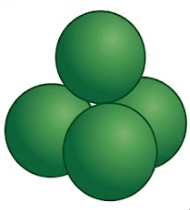
\includegraphics[width=0.2\textwidth]{Problem_2/Image/P2_I4.png}
        \caption{Cách hai lớp phân tử xếp chồng lên nhau}
        \label{P2_I4}   
    \end{figure}
    Nhằm xác định số liên kết bị gãy, ta cần tìm mật độ số liên kết trên đơn vị diện tích của cấu hình này. Song, trong trường hợp này, vì ta không thể chia cắt các phân tử thành từng lớp song song với nhau, kết quả ước lượng được sẽ phụ thuộc vào cách ta "cắt"; dù thường thì hệ số tìm được sẽ không chênh nhau quá $10\%$. Sau đây ta sẽ chỉ trình bày một cách tiếp cận:\newline
    Ô đơn vị của một phân tử là một khối thập nhị diện đều mà mặt cắt ngang chính là một hình lục giác, do đó ta có được hình ảnh mặt cắt ngang hai lớp phân tử chồng lên nhau như \figref{P2_tikz3}. Việc bẻ gãy liên kết đã xảy ra sẽ được coi như tách rời các lớp chồng lên nhau như vậy.\newline
    Dễ dàng tính được diện tích mặt cắt ngang một ô đơn vị, một hình lục giác đều cạnh $2r/\sqrt{3}$, là bằng $2\sqrt 3 r^2$, nên mật độ phân tử trên đơn vị diện tích lầ $1/(2\sqrt3 r^2)$.
    Một phân tử ở lớp dưới sẽ liên kết với $3$ phân tử ở lớp trên, nhưng số liên kết hiệu dụng chỉ là $3/2$. Như vậy mật độ số liên kết chính là \begin{equation}
        \sigma=\frac{3}{2}\times \frac{1}{2\sqrt{3}r^2}=\frac{\sqrt{3}}{4r^2}.
    \end{equation}
    Qua đó số liên kết bị bẻ gãy bằng \begin{equation}
        N=lc\sigma=\frac{\sqrt{3}lc}{4r^2}\approx 5.6\times 10^{14}\text{~liên kết}.
    \end{equation}
    \item[(e)] Thay $A=12$, kết quả thu được là \begin{equation}
        E_b =\frac{M_{SiO_2}L}{6N_A}=1.7\times 10^{-19}\text{~J/liên kết}.
    \end{equation} Kết quả này đơn giản là bằng một nửa năng lượng liên kết của cấu hình hệ lập phương, vì biến số duy nhất là $A$: sự bền vững của cấu trúc phụ thuộc trực tiếp và duy nhất vào số phân tử một phân tử tiếp xúc trực tiếp; số phân tử "giữ lấy" một phân tử càng nhiều, năng lượng cần để bứt nó ra khỏi hệ lại càng nhỏ. 
    \item[(f)] Phương trình cân bằng năng lượng không thay đổi, thay thế $E_b$ và $N$ cho trường hợp này, ta thu được hiệu suất \begin{equation}
        H=\frac{NE_b}{E}=0.26\%.
    \end{equation}
    Rõ ràng là năng lượng cần thiết để bẻ gãy liên kết trong hệ lục giác xếp chặt nhỏ hơn đáng kể so với hệ lập phương, dù số liên kết cần phải bẻ gãy lớn hơn hẳn.
\end{enumerate}
Thực tế, cấu trúc tinh thể của $\mathrm{SiO_2}$ trong tự nhiên không chính xác là hệ lập phương và hệ lục giác xếp chặt, đó chỉ là lần lượt hai gần đúng cho $\alpha$-quartz và cristobalite. Hơn nữa, khối lượng riêng của hai loại trên cũng không bằng nhau, ta có thể kiểm chứng lại điều này với giả thiết bán kính phân tử trong cả hai trường hợp là một. Sử dụng giá trị của $\rho$ như đã cho chung cho cả hai cấu trúc chỉ là một ước lượng thô không chính xác. Ý nghĩa của các ước lượng trên như vậy chỉ nhằm khảo sát định tính một số tính chất thú vị của hiện tượng thông qua các mô hình đơn giản. Song hy vọng bài toán này vẫn mang tới cho các bạn vài điều bổ ích và sảng khoái.
\vspace{0.5cm}

\noindent \textbf{\large Phổ điểm}
\begin{center}
\renewcommand{\arraystretch}{1.5}
\begin{tabularx}{\textwidth}{|c|X|c|}
\hline
\textbf{Phần} & \textbf{Nội dung} & \textbf{Điểm thành phần} \\ \hline
a &Ước lượng gần đúng chiều dài rãnh gãy với sai số không quá $5mm$ . & 0.25 \\ \cline{2-3} 
&Xác định đúng kích thước ô cơ sở. & 0.25 \\ \cline{2-3} 
 & Ước lượng số liên kết bị bẻ gãy với sai số cỡ $10\%$. & 0.25 \\ \hline
b &Thiết lập biểu thức tính tổng số liên kết đối với hệ lập phương . & 0.25 \\ \cline{2-3} 
&Tổng quát hoá cách chứng minh trên với mọi cấu hình. & 0.25 \\ \cline{2-3} 
 & Nêu ra ý nghĩa của ẩn nhiệt hoá hơi và tính toán đúng năng lượng liên kết. & 0.25 \\ \hline
c & Nêu được tổng năng lượng ban đầu và tính đúng tỷ lệ. & 0.5 \\ \hline
d &Xác định đúng kích thước phân tử. & 0.25 \\ \cline{2-3} 
&Đưa ra một cách xác định mật độ liên kết. & 0.25\\ \cline{2-3} 
 &Tính đúng số liên kết bị bẻ gãy . & 0.25 \\ \hline
 e & Nêu ra giá trị của $A$ và tính được đúng là năng lượng liên kết. & 0.75 \\ \hline
f & Thay số đúng để tính đúng giá trị cần tìm. & 0.5 \\ \hline
\multicolumn{2}{|r|}{\textbf{Tổng điểm}} & \textbf{4.0} \\ \hline
\end{tabularx}
\end{center}